\documentclass[12pt, twoside]{article}
\usepackage[francais]{babel}
\usepackage[T1]{fontenc}
\usepackage[latin1]{inputenc}
\usepackage[left=5mm, right=5mm, top=3mm, bottom=3mm]{geometry}
\usepackage{float}
\usepackage{graphicx}
\usepackage{array}
\usepackage{multirow}
\usepackage{amsmath,amssymb,mathrsfs}
\usepackage{soul}
\usepackage{textcomp}
\usepackage{eurosym}
 \usepackage{variations}
\usepackage{tabvar}


\pagestyle{empty}

\begin{document}


\section*{\center{Devoir maison 9}}


\medskip





\fbox{

\begin{minipage}{18cm}
\textit{Devoir � rendre sur feuille grand format petits
carreaux pour le \textbf{mardi 22 mai 2012}. La justification et la \textbf{r�daction} seront prises en
 compte dans le bar�me.}
\end{minipage}
}

\medskip




\ul{Exercice 1} \textit{(4 points)} \qquad 
Sur la figure suivante, AEFG est un carr� de c�t� $a$ et ABCD est un rectangle.

\enskip

\begin{tabular}{cc}
\begin{minipage}{155mm}

 
\begin{enumerate}
  \item P�rim�tre de ABCD:
  
  \begin{enumerate}
    \item D�terminer l'expression r�duite donnant le p�rim�tre du rectangle
    ABCD.
    \item Pour a=6cm, calculer le p�rim�tre du rectangle ABCD.
  \end{enumerate}

\item Aire de ABCD:

 \begin{enumerate}
   \item Exprimer l'aire de ABCD sous la forme d'une expression factoris�e.
   \item D�velopper et r�duire l'expression obtenue � la question 2.a)
   \item Pour a=6cm, calculer l'aire du rectangle ABCD de deux fa�ons
   diff�rentes.
 \end{enumerate}
 
\end{enumerate}

\end{minipage}
&
\begin{minipage}{4cm}
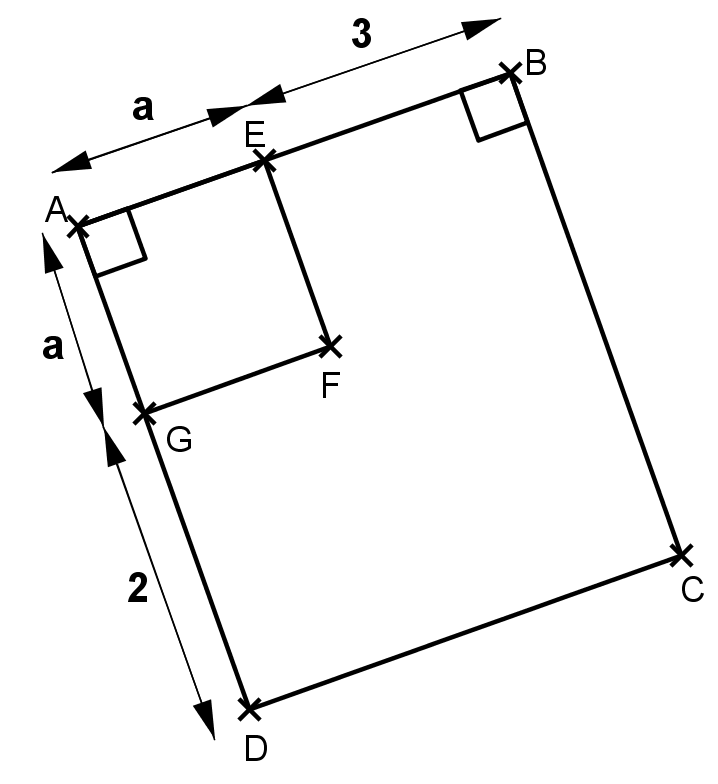
\includegraphics[width=4cm]{images/ex2.png}  
\end{minipage}
\end{tabular}

\bigskip

\ul{Exercice 2} \textit{(2 points)} \qquad 
R�duire l'expression suivante:
A=(3t-6)(-5-t)+4(2t+7)

\bigskip


\ul{Exercice 3} \textit{(3 points)}

\enskip

Pascal ach�te 7 pains au chocolat et 4 croissants. Un croissant co�te $y$
\euro. Un pain au chocolat co�te 0,20 \euro de plus qu'un croissant.

\begin{enumerate}
  \item Exprimer le prix d'un pain au chocolat en fonction de $y$.
  
  \item  Ecrire en fonction de $y$ la d�pense totale de Pascal.
  \item D�velopper et r�duire l'expression trouv�e.
  \item Si un croissant co�te 0,80 \euro, combien doit payer Pascal?
\end{enumerate}

\medskip

\ul{Exercice 4} \textit{(4 points)}

\begin{tabular}{cc}
\begin{minipage}{9cm}

En utilisant les informations port�es sur la figure:


\begin{enumerate}
  \item Calculer MN.
  \item En d�duire BC.
\end{enumerate} 
\end{minipage}
&
\begin{minipage}{9cm}
\begin{center}
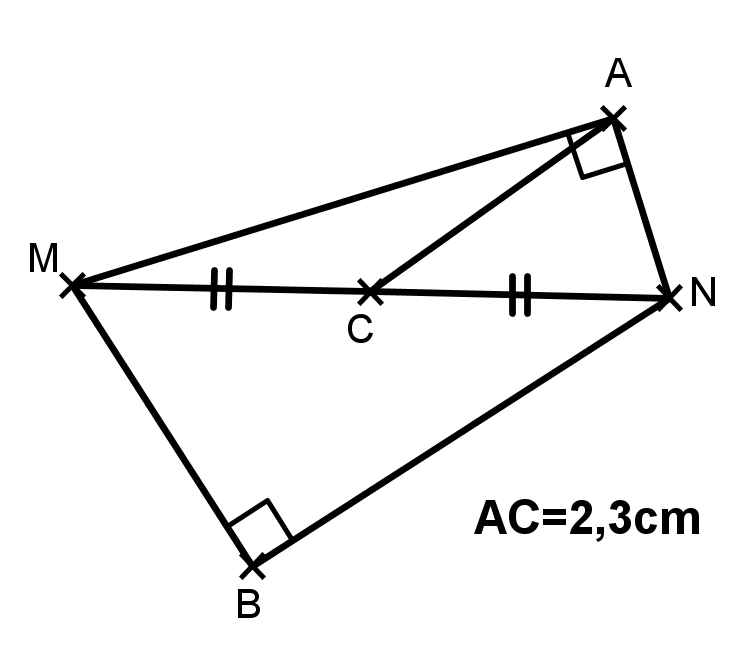
\includegraphics[width=4cm]{images/ex2bis.png}
\end{center}

\end{minipage}
\end{tabular}

\medskip

\ul{Exercice 5} \textit{(3,5 points)}


\begin{tabular}{cr} 
\begin{minipage}{11cm}

Construire un point P tels que les triangles ABP et CDP soient rectangles en P.
Justifier votre r�ponse.

\enskip

(\textit{La construction se fera sur la photocopie et les explications seront
not�es sur votre feuille.})


\end{minipage}
&
\begin{minipage}{7cm}
\begin{center}
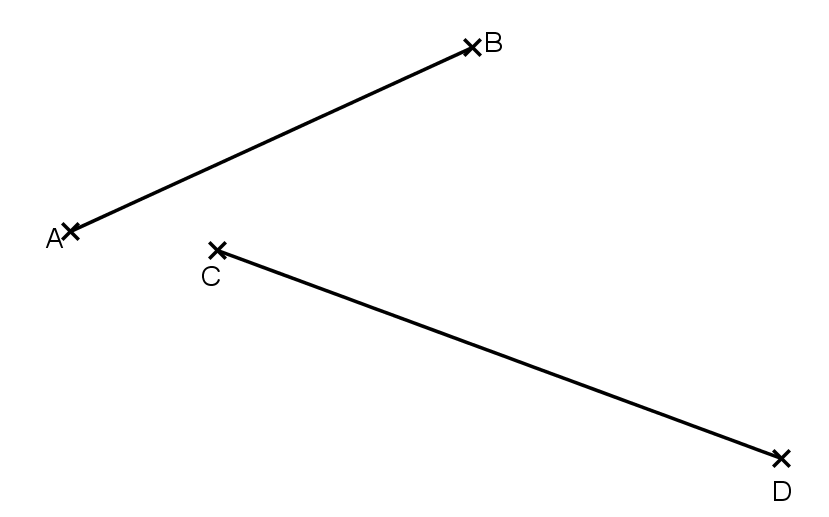
\includegraphics[width=65mm]{images/ex4.png}
\end{center}
\end{minipage} 
\end{tabular}

\medskip

\ul{Exercice 6} \textit{(4,5 points)}


\enskip

 Soit [IJ] un segment de longueur 8cm. $\mathcal{C}$
est le cercle de diam�tre [IJ]. Le point K appartient au cercle $\mathcal{C}$
et v�rifie JK=3,5cm.



\begin{enumerate}
  \item Faire la figure.
  \item D�montrer que le triangle IJK est rectangle en K.
  \item Calculer JK (on donnera le r�sultat arrondi au mm). Justifier votre
  r�ponse.
\end{enumerate}


\end{document}
